% Options for packages loaded elsewhere
\PassOptionsToPackage{unicode}{hyperref}
\PassOptionsToPackage{hyphens}{url}
\PassOptionsToPackage{dvipsnames,svgnames,x11names}{xcolor}
%
\documentclass[
  11pt,
  a4paper,
]{article}
\usepackage{amsmath,amssymb}
\usepackage{iftex}
\ifPDFTeX
  \usepackage[T1]{fontenc}
  \usepackage[utf8]{inputenc}
  \usepackage{textcomp} % provide euro and other symbols
\else % if luatex or xetex
  \usepackage{unicode-math} % this also loads fontspec
  \defaultfontfeatures{Scale=MatchLowercase}
  \defaultfontfeatures[\rmfamily]{Ligatures=TeX,Scale=1}
\fi
\usepackage{lmodern}
\ifPDFTeX\else
  % xetex/luatex font selection
  \setmainfont[]{DejaVu Serif}
  \setmonofont[]{DejaVu Sans Mono}
\fi
% Use upquote if available, for straight quotes in verbatim environments
\IfFileExists{upquote.sty}{\usepackage{upquote}}{}
\IfFileExists{microtype.sty}{% use microtype if available
  \usepackage[]{microtype}
  \UseMicrotypeSet[protrusion]{basicmath} % disable protrusion for tt fonts
}{}
\makeatletter
\@ifundefined{KOMAClassName}{% if non-KOMA class
  \IfFileExists{parskip.sty}{%
    \usepackage{parskip}
  }{% else
    \setlength{\parindent}{0pt}
    \setlength{\parskip}{6pt plus 2pt minus 1pt}}
}{% if KOMA class
  \KOMAoptions{parskip=half}}
\makeatother
\usepackage{xcolor}
\usepackage[margin=2.5cm]{geometry}
\usepackage{color}
\usepackage{fancyvrb}
\newcommand{\VerbBar}{|}
\newcommand{\VERB}{\Verb[commandchars=\\\{\}]}
\DefineVerbatimEnvironment{Highlighting}{Verbatim}{commandchars=\\\{\}}
% Add ',fontsize=\small' for more characters per line
\newenvironment{Shaded}{}{}
\newcommand{\AlertTok}[1]{\textcolor[rgb]{1.00,0.00,0.00}{\textbf{#1}}}
\newcommand{\AnnotationTok}[1]{\textcolor[rgb]{0.38,0.63,0.69}{\textbf{\textit{#1}}}}
\newcommand{\AttributeTok}[1]{\textcolor[rgb]{0.49,0.56,0.16}{#1}}
\newcommand{\BaseNTok}[1]{\textcolor[rgb]{0.25,0.63,0.44}{#1}}
\newcommand{\BuiltInTok}[1]{\textcolor[rgb]{0.00,0.50,0.00}{#1}}
\newcommand{\CharTok}[1]{\textcolor[rgb]{0.25,0.44,0.63}{#1}}
\newcommand{\CommentTok}[1]{\textcolor[rgb]{0.38,0.63,0.69}{\textit{#1}}}
\newcommand{\CommentVarTok}[1]{\textcolor[rgb]{0.38,0.63,0.69}{\textbf{\textit{#1}}}}
\newcommand{\ConstantTok}[1]{\textcolor[rgb]{0.53,0.00,0.00}{#1}}
\newcommand{\ControlFlowTok}[1]{\textcolor[rgb]{0.00,0.44,0.13}{\textbf{#1}}}
\newcommand{\DataTypeTok}[1]{\textcolor[rgb]{0.56,0.13,0.00}{#1}}
\newcommand{\DecValTok}[1]{\textcolor[rgb]{0.25,0.63,0.44}{#1}}
\newcommand{\DocumentationTok}[1]{\textcolor[rgb]{0.73,0.13,0.13}{\textit{#1}}}
\newcommand{\ErrorTok}[1]{\textcolor[rgb]{1.00,0.00,0.00}{\textbf{#1}}}
\newcommand{\ExtensionTok}[1]{#1}
\newcommand{\FloatTok}[1]{\textcolor[rgb]{0.25,0.63,0.44}{#1}}
\newcommand{\FunctionTok}[1]{\textcolor[rgb]{0.02,0.16,0.49}{#1}}
\newcommand{\ImportTok}[1]{\textcolor[rgb]{0.00,0.50,0.00}{\textbf{#1}}}
\newcommand{\InformationTok}[1]{\textcolor[rgb]{0.38,0.63,0.69}{\textbf{\textit{#1}}}}
\newcommand{\KeywordTok}[1]{\textcolor[rgb]{0.00,0.44,0.13}{\textbf{#1}}}
\newcommand{\NormalTok}[1]{#1}
\newcommand{\OperatorTok}[1]{\textcolor[rgb]{0.40,0.40,0.40}{#1}}
\newcommand{\OtherTok}[1]{\textcolor[rgb]{0.00,0.44,0.13}{#1}}
\newcommand{\PreprocessorTok}[1]{\textcolor[rgb]{0.74,0.48,0.00}{#1}}
\newcommand{\RegionMarkerTok}[1]{#1}
\newcommand{\SpecialCharTok}[1]{\textcolor[rgb]{0.25,0.44,0.63}{#1}}
\newcommand{\SpecialStringTok}[1]{\textcolor[rgb]{0.73,0.40,0.53}{#1}}
\newcommand{\StringTok}[1]{\textcolor[rgb]{0.25,0.44,0.63}{#1}}
\newcommand{\VariableTok}[1]{\textcolor[rgb]{0.10,0.09,0.49}{#1}}
\newcommand{\VerbatimStringTok}[1]{\textcolor[rgb]{0.25,0.44,0.63}{#1}}
\newcommand{\WarningTok}[1]{\textcolor[rgb]{0.38,0.63,0.69}{\textbf{\textit{#1}}}}
\usepackage{longtable,booktabs,array}
\usepackage{calc} % for calculating minipage widths
% Correct order of tables after \paragraph or \subparagraph
\usepackage{etoolbox}
\makeatletter
\patchcmd\longtable{\par}{\if@noskipsec\mbox{}\fi\par}{}{}
\makeatother
% Allow footnotes in longtable head/foot
\IfFileExists{footnotehyper.sty}{\usepackage{footnotehyper}}{\usepackage{footnote}}
\makesavenoteenv{longtable}
\usepackage{graphicx}
\makeatletter
\def\maxwidth{\ifdim\Gin@nat@width>\linewidth\linewidth\else\Gin@nat@width\fi}
\def\maxheight{\ifdim\Gin@nat@height>\textheight\textheight\else\Gin@nat@height\fi}
\makeatother
% Scale images if necessary, so that they will not overflow the page
% margins by default, and it is still possible to overwrite the defaults
% using explicit options in \includegraphics[width, height, ...]{}
\setkeys{Gin}{width=\maxwidth,height=\maxheight,keepaspectratio}
% Set default figure placement to htbp
\makeatletter
\def\fps@figure{htbp}
\makeatother
\setlength{\emergencystretch}{3em} % prevent overfull lines
\providecommand{\tightlist}{%
  \setlength{\itemsep}{0pt}\setlength{\parskip}{0pt}}
\setcounter{secnumdepth}{-\maxdimen} % remove section numbering
\ifLuaTeX
  \usepackage{selnolig}  % disable illegal ligatures
\fi
\IfFileExists{bookmark.sty}{\usepackage{bookmark}}{\usepackage{hyperref}}
\IfFileExists{xurl.sty}{\usepackage{xurl}}{} % add URL line breaks if available
\urlstyle{same}
\hypersetup{
  pdftitle={Pad Ring Generation with LibreLane for the IHP SG13G2 Process},
  pdfauthor={Koen Van Caekenberghe, Ph.D.~--- ChipDesign B.V. --- info@chipdesign.be},
  colorlinks=true,
  linkcolor={NavyBlue},
  filecolor={Maroon},
  citecolor={Blue},
  urlcolor={NavyBlue},
  pdfcreator={LaTeX via pandoc}}

\title{Pad Ring Generation with LibreLane for the IHP SG13G2 Process}
\usepackage{etoolbox}
\makeatletter
\providecommand{\subtitle}[1]{% add subtitle to \maketitle
  \apptocmd{\@title}{\par {\large #1 \par}}{}{}
}
\makeatother
\subtitle{Method, driver script (line by line), and the generated
pad-ring layout of the chip\_top demonstrator}
\author{Koen Van Caekenberghe, Ph.D.~--- ChipDesign B.V. ---
\href{mailto:info@chipdesign.be}{\nolinkurl{info@chipdesign.be}}}
\date{2026-07-22}

\begin{document}
\maketitle

{
\hypersetup{linkcolor=}
\setcounter{tocdepth}{3}
\tableofcontents
}
\hypertarget{scope-and-method}{%
\section{1. Scope and method}\label{scope-and-method}}

This report documents how a \textbf{pad ring} is generated for a chip on
the \textbf{IHP SG13G2} 130 nm open-source process using
\textbf{LibreLane} --- the successor to OpenLane 2. A pad ring is the
outer belt of I/O cells that surrounds the core: it carries the bond
pads, the ESD structures, the level shifters between the 1.2 V core and
the 3.3 V outside world, and the power/ground rails that ring the die.
Without it, a hardened core has nothing to be wired or probed through.

The approach here is \textbf{fully integrated}: rather than assembling
the ring in a separate GDS tool, we describe the ring \emph{structurally
in Verilog} (one I/O-cell instance per chip pin), hand that top level to
LibreLane's \textbf{\texttt{Chip} flow}, and let its
\textbf{\texttt{OpenROAD.PadRing}} step place the pads, corners and
fillers and connect the ring rails by abutment. The same netlist that
defines the ring is therefore the one that is later placed, routed and
verified --- there is no manual GDS step to keep in sync.

The worked example is \texttt{chip\_top}, a 32-pad ring around a small
placeholder core (\texttt{demo\_core}). Everything below is reproducible
from the files in this repository with a single command (§4).

\begin{longtable}[]{@{}
  >{\raggedright\arraybackslash}p{(\columnwidth - 2\tabcolsep) * \real{0.5000}}
  >{\raggedright\arraybackslash}p{(\columnwidth - 2\tabcolsep) * \real{0.5000}}@{}}
\toprule\noalign{}
\begin{minipage}[b]{\linewidth}\raggedright
Item
\end{minipage} & \begin{minipage}[b]{\linewidth}\raggedright
Value
\end{minipage} \\
\midrule\noalign{}
\endhead
\bottomrule\noalign{}
\endlastfoot
Process & IHP SG13G2 (130 nm), \texttt{PDK=ihp-sg13g2} \\
Tool & LibreLane 3.1, flow \texttt{Chip}, step
\texttt{OpenROAD.PadRing} \\
I/O library & \texttt{sg13g2\_io} (\texttt{libs.ref/sg13g2\_io}) \\
Pad cell footprint & 80 µm (along ring) × 180 µm (deep) \\
Corner cell & 180 × 180 µm \\
Pad-to-edge (seal-ring) spacing &
\texttt{PAD\_EDGE\_SPACING\ =\ 140\ µm} \\
Pad pitch & \textbf{150 µm}, uniform on all four sides \\
Die & 1910 × 1910 µm, 8 pads per side \\
Result & 32 I/O pads + 4 corners + 72 fillers, ring closed by
abutment \\
\end{longtable}

\begin{center}\rule{0.5\linewidth}{0.5pt}\end{center}

\hypertarget{the-ihp-sg13g2-io-cell-library}{%
\section{2. The IHP SG13G2 I/O cell
library}\label{the-ihp-sg13g2-io-cell-library}}

The pad ring is built exclusively from cells in
\texttt{libs.ref/sg13g2\_io}. LibreLane learns about them automatically:
the PDK ships a LibreLane configuration
(\texttt{libs.tech/librelane/sg13g2\_io/config.tcl}) that registers the
pad LEF/GDS/Verilog, the placement \textbf{sites}
(\texttt{sg13g2\_ioSite}, \texttt{sg13g2\_cornerSite}), the corner and
filler cell names, and the 140 µm edge spacing. The relevant cell
classes are:

\begin{longtable}[]{@{}
  >{\raggedright\arraybackslash}p{(\columnwidth - 4\tabcolsep) * \real{0.3333}}
  >{\raggedright\arraybackslash}p{(\columnwidth - 4\tabcolsep) * \real{0.3333}}
  >{\raggedright\arraybackslash}p{(\columnwidth - 4\tabcolsep) * \real{0.3333}}@{}}
\toprule\noalign{}
\begin{minipage}[b]{\linewidth}\raggedright
Class
\end{minipage} & \begin{minipage}[b]{\linewidth}\raggedright
Cells
\end{minipage} & \begin{minipage}[b]{\linewidth}\raggedright
Purpose
\end{minipage} \\
\midrule\noalign{}
\endhead
\bottomrule\noalign{}
\endlastfoot
Input & \texttt{sg13g2\_IOPadIn} & pad → core receiver \\
Output & \texttt{sg13g2\_IOPadOut\{4,16,30\}mA} & core → pad driver,
three drive strengths \\
Tri-state & \texttt{sg13g2\_IOPadTriOut\{4,16,30\}mA} & driver with
output-enable \\
Bidirectional & \texttt{sg13g2\_IOPadInOut\{4,16,30\}mA} & driver +
receiver + enable \\
Analog & \texttt{sg13g2\_IOPadAnalog} & direct pad ↔ core analog
connection \\
Power / ground & \texttt{sg13g2\_IOPad\{Vdd,Vss,IOVdd,IOVss\}} & core
(1.2 V) and I/O (3.3 V) supply pads \\
Corner & \texttt{sg13g2\_Corner} & die-corner cell that turns the ring
90° \\
Filler & \texttt{sg13g2\_Filler\{200…10000\}} & close the gaps between
pads and continue the rails \\
\end{longtable}

A note on \textbf{bond pads}: the IHP I/O cells already carry their
wire-bond opening \emph{inside} the pad cell (the Liberty attribute
\texttt{bond\_pads\ :\ 1} is set on every \texttt{sg13g2\_IOPad*}).
There is no separate bond-pad cell in the PDK. The bond wire therefore
lands directly on the pad cell, and the flow is told not to look for a
stand-alone bond-pad master (§6, \texttt{PAD\_BONDPAD\_NAME:\ null}).

\begin{center}\rule{0.5\linewidth}{0.5pt}\end{center}

\hypertarget{how-the-pad-ring-is-placed}{%
\section{3. How the pad ring is
placed}\label{how-the-pad-ring-is-placed}}

The \texttt{OpenROAD.PadRing} step runs the PDK-agnostic algorithm in
\texttt{librelane/scripts/openroad/common/pad\_cfg.tcl}. Conceptually,
for each of the four sides it:

\begin{enumerate}
\def\labelenumi{\arabic{enumi}.}
\tightlist
\item
  builds an I/O placement row inset from the die edge by
  \texttt{PAD\_EDGE\_SPACING} (140 µm), leaving room for the seal ring;
\item
  sums the widths of the pads assigned to that side and checks they fit;
\item
  distributes the free space \emph{evenly} --- the inter-pad gap is
  rounded down to the 1 µm minimum filler granularity, and the two end
  gaps to the corners absorb the remainder;
\item
  places each pad instance at the computed coordinate with the correct
  rotation for that side;
\item
  drops the four \texttt{sg13g2\_Corner} cells and back-fills every
  remaining gap with the largest fitting \texttt{sg13g2\_Filler*};
\item
  calls \texttt{connect\_by\_abutment}, so the power, ground and ESD
  rails that run through every cell join into four continuous rings
  simply because the cells touch.
\end{enumerate}

The engineer therefore controls only two things: \textbf{which pad
instances exist} (the Verilog, §5) and \textbf{which side each one sits
on, in what order} (the \texttt{PAD\_*} lists, §6). The spacing is
computed.

\textbf{Setting the pad pitch.} Because the pads are spread evenly, the
centre-to-centre pitch is not a direct configuration knob --- it
\emph{emerges} from the die size. For a target pitch \(p\) with pad
width \(w_{pad}\) and \(N\) pads on a side, the inter-pad gap must be
\(g = p - w_{pad}\), and the die side that produces it exactly is

\[\mathrm{side} = 2\cdot 140 + 2\cdot 180 + N\,w_{pad} + (N{+}1)\,g\]

For the required \textbf{150 µm pitch} with 80 µm pads and \(N = 8\):
\(g = 70\) µm and side
\(= 280 + 360 + 640 + 9 \cdot 70 = \mathbf{1910}\) µm. Two divisibility
conditions make the pitch \emph{exact} rather than approximate: the
algorithm floors the gap to the 1 µm site width (\(630 / 9 = 70\)
exactly, no loss), and the two end gaps \((630 - 7\cdot 70)/2 = 70\) µm
land on the site grid. Off-grid choices are silently floored --- the
pitch then comes out slightly below target --- so the die should always
be derived from the pitch, not the other way around.

\begin{center}\rule{0.5\linewidth}{0.5pt}\end{center}

\hypertarget{the-generation-script-line-by-line}{%
\section{4. The generation script, line by
line}\label{the-generation-script-line-by-line}}

The whole flow is driven by \texttt{gen\_padring.sh}:

\begin{Shaded}
\begin{Highlighting}[]
 \ExtensionTok{1}  \CommentTok{\#!/bin/bash}
 \ExtensionTok{2}  \CommentTok{\# gen\_padring.sh — generate the pad ring with LibreLane (IHP SG13G2)}
 \ExtensionTok{3}\NormalTok{  set }\AttributeTok{{-}euo}\NormalTok{ pipefail}
 \ExtensionTok{4}\NormalTok{  cd }\StringTok{"}\VariableTok{$(}\FunctionTok{dirname} \StringTok{"}\VariableTok{$0}\StringTok{"}\VariableTok{)}\StringTok{"}
 \ExtensionTok{5}
 \ExtensionTok{6}  \CommentTok{\# {-}{-}{-} 1. Environment: PDK location, tool paths {-}{-}{-}}
 \ExtensionTok{7}\NormalTok{  . ./env.sh}
 \ExtensionTok{8}
 \ExtensionTok{9}  \CommentTok{\# {-}{-}{-} 2. Run the Chip flow up to the pad{-}ring step {-}{-}{-}}
\ExtensionTok{10}\NormalTok{  librelane config.yaml }\DataTypeTok{\textbackslash{}}
\NormalTok{11      }\AttributeTok{{-}{-}pdk} \StringTok{"}\VariableTok{$PDK}\StringTok{"} \AttributeTok{{-}{-}pdk{-}root} \StringTok{"}\VariableTok{$PDK\_ROOT}\StringTok{"} \AttributeTok{{-}{-}manual{-}pdk} \DataTypeTok{\textbackslash{}}
\NormalTok{12      }\AttributeTok{{-}{-}to}\NormalTok{ OpenROAD.PadRing }\DataTypeTok{\textbackslash{}}
\NormalTok{13      }\StringTok{"}\VariableTok{$@}\StringTok{"}
\ExtensionTok{14}
\ExtensionTok{15}  \CommentTok{\# {-}{-}{-} 3. Report where the result landed {-}{-}{-}}
\ExtensionTok{16}\NormalTok{  RUN=}\VariableTok{$(}\FunctionTok{ls} \AttributeTok{{-}dt}\NormalTok{ runs/RUN\_}\PreprocessorTok{*} \KeywordTok{|} \FunctionTok{head} \AttributeTok{{-}1}\VariableTok{)}
\ExtensionTok{17}\NormalTok{  echo }\StringTok{"Pad ring written to: }\VariableTok{$RUN}\StringTok{/16{-}openroad{-}padring/chip\_top.def"}
\end{Highlighting}
\end{Shaded}

\textbf{Line 3} --- \texttt{set\ -euo\ pipefail} makes the script fail
fast: abort on any command error (\texttt{-e}), on an undefined variable
(\texttt{-u}), and on a failure anywhere in a pipeline
(\texttt{-o\ pipefail}). A silent half-finished pad ring is worse than a
clean stop.

\textbf{Line 4} --- \texttt{cd} to the script's own directory so the
relative paths in \texttt{config.yaml} (which use LibreLane's
\texttt{dir::} prefix) resolve regardless of where the script is invoked
from.

\textbf{Line 7} --- source \texttt{env.sh}, the single place where the
environment is configured. It exports \texttt{PDK\_ROOT} and
\texttt{PDK} (defaulting to a standard installation, both overridable
from the caller's environment) and prepends common EDA tool locations to
\texttt{PATH} \emph{when they exist} --- many setups do not expose
\texttt{yosys}, \texttt{openroad} and \texttt{klayout} to
non-interactive shells, and without this LibreLane's sub-processes fail
with \emph{``command not found''}. On systems where the tools are
already on \texttt{PATH} the loop is a no-op, so the script stays
portable.

\textbf{Line 10} --- invoke LibreLane on the design's
\texttt{config.yaml}. Everything about \emph{what} is built lives in
that file (§6); the command line only says \emph{how far} and
\emph{against which PDK}.

\textbf{Line 11} ---
\texttt{-\/-pdk\ …\ -\/-pdk-root\ …\ -\/-manual-pdk}. The critical flag
is \textbf{\texttt{-\/-manual-pdk}}: it tells LibreLane to use the PDK
already on disk instead of trying to download a version-pinned copy
through \texttt{ciel}. Without it the run can die trying to write into a
read-only version-managed PDK cache.

\textbf{Line 12} --- \textbf{\texttt{-\/-to\ OpenROAD.PadRing}} stops
the flow immediately after the pad ring is placed. This is the
``pad-ring only'' mode: synthesis → floorplan → power-net setup →
\textbf{pad ring}, then halt, so pad placement can be inspected and
iterated in seconds without paying for full place-and-route. Dropping
this flag runs the complete \texttt{Chip} flow through to a signed-off
chip GDS (seal ring, filler, density and antenna checks included).

\textbf{Line 13} --- \texttt{"\$@"} forwards any extra arguments to
LibreLane (e.g.~\texttt{-\/-to\ Odb.SetPowerConnections} to stop even
earlier, or nothing to run to \texttt{PadRing}).

\textbf{Lines 16--17} --- find the newest run directory and print the
path of the emitted pad-ring DEF --- the artifact rendered in §7.

Run it with:

\begin{Shaded}
\begin{Highlighting}[]
\ExtensionTok{./gen\_padring.sh}
\end{Highlighting}
\end{Shaded}

\begin{center}\rule{0.5\linewidth}{0.5pt}\end{center}

\hypertarget{defining-the-ring-in-verilog-excerpt-line-by-line}{%
\section{5. Defining the ring in Verilog (excerpt, line by
line)}\label{defining-the-ring-in-verilog-excerpt-line-by-line}}

The pad ring's \emph{contents} are one I/O-cell instantiation per pin in
the chip top (\texttt{src/chip\_top.v}). The instance \textbf{names}
chosen here are exactly the handles the placer uses in §6. A
representative slice:

\begin{Shaded}
\begin{Highlighting}[]
 \DecValTok{1}  \OperatorTok{(}\NormalTok{* keep *}\OperatorTok{)}\NormalTok{ sg13g2\_IOPadIOVdd sg13g2\_IOPad\_iovdd\_w }\OperatorTok{(}
 \DecValTok{2}  \OtherTok{\textasciigrave{}ifdef}\NormalTok{ USE\_POWER\_PINS}
 \DecValTok{3}\NormalTok{      .vss}\OperatorTok{(}\NormalTok{VSS}\OperatorTok{),}\NormalTok{ .vdd}\OperatorTok{(}\NormalTok{VDD}\OperatorTok{),}\NormalTok{ .iovss}\OperatorTok{(}\NormalTok{IOVSS}\OperatorTok{),}\NormalTok{ .iovdd}\OperatorTok{(}\NormalTok{IOVDD}\OperatorTok{)}
 \DecValTok{4}  \OtherTok{\textasciigrave{}endif}
 \DecValTok{5}  \OperatorTok{);}
 \DecValTok{6}
 \DecValTok{7}\NormalTok{  sg13g2\_IOPadIn sg13g2\_IOPad\_io\_clk }\OperatorTok{(}
 \DecValTok{8}\NormalTok{      .p2c}\OperatorTok{(}\NormalTok{clk\_i}\OperatorTok{),}\NormalTok{ .pad}\OperatorTok{(}\NormalTok{clk\_PAD}\OperatorTok{)}
 \DecValTok{9}  \OperatorTok{);}
\DecValTok{10}
\DecValTok{11}\NormalTok{  sg13g2\_IOPadOut30mA sg13g2\_IOPad\_io\_done }\OperatorTok{(}
\DecValTok{12}\NormalTok{      .c2p}\OperatorTok{(}\NormalTok{done\_o}\OperatorTok{),}\NormalTok{ .pad}\OperatorTok{(}\NormalTok{done\_PAD}\OperatorTok{)}
\DecValTok{13}  \OperatorTok{);}
\DecValTok{14}
\DecValTok{15}\NormalTok{  sg13g2\_IOPadInOut30mA sg13g2\_IOPad\_io\_gpio }\OperatorTok{(}
\DecValTok{16}\NormalTok{      .c2p}\OperatorTok{(}\NormalTok{gpio\_out}\OperatorTok{),}\NormalTok{ .c2p\_en}\OperatorTok{(}\NormalTok{gpio\_oe}\OperatorTok{),}\NormalTok{ .p2c}\OperatorTok{(}\NormalTok{gpio\_in}\OperatorTok{),}\NormalTok{ .pad}\OperatorTok{(}\NormalTok{gpio\_PAD}\OperatorTok{)}
\DecValTok{17}  \OperatorTok{);}
\end{Highlighting}
\end{Shaded}

\textbf{Line 1} --- a \textbf{power pad}. \texttt{(*\ keep\ *)} stops
synthesis from optimising the cell away: it has no logic function, only
supply connections, so without the attribute Yosys would delete it. The
instance name \texttt{sg13g2\_IOPad\_iovdd\_w} is what appears in
\texttt{PAD\_WEST}.

\textbf{Lines 2--4} --- the four ring supply nets (\texttt{vdd},
\texttt{vss}, \texttt{iovdd}, \texttt{iovss}) are wired only under the
\texttt{USE\_POWER\_PINS} macro. During logic synthesis the macro is off
and the pins float; the physical rails are joined later by
\texttt{connect\_by\_abutment}, and the global power connections tie
them to the supply nets. This is the standard LibreLane power-pad idiom.

\textbf{Lines 7--9} --- an \textbf{input pad}. \texttt{sg13g2\_IOPadIn}
has two signal pins: \texttt{pad} is the external bond pad (a top-level
port of the chip), and \texttt{p2c} (``pad-to-core'') is the received
signal handed to the core net \texttt{clk\_i}.

\textbf{Lines 11--13} --- an \textbf{output pad}, drive strength 30 mA.
Here the direction reverses: the core drives \texttt{c2p}
(``core-to-pad'') and the cell drives the external \texttt{pad}.

\textbf{Lines 15--17} --- a \textbf{bidirectional pad}. It combines both
directions plus an output-enable: \texttt{c2p}/\texttt{c2p\_en} drive
the pad when enabled, and \texttt{p2c} always returns the pad value to
the core --- the three-wire decomposition of an \texttt{inout}.

Buses of pads are built with a \texttt{generate} loop; the resulting
instance names take the hierarchical form
\texttt{sg13g2\_IOPad\_dout{[}0{]}.sg13g2\_IOPad\_io\_dout}, which is
why those entries are bracket-escaped in the configuration.

\begin{center}\rule{0.5\linewidth}{0.5pt}\end{center}

\hypertarget{assigning-pads-to-sides-in-config.yaml-line-by-line}{%
\section{\texorpdfstring{6. Assigning pads to sides in
\texttt{config.yaml} (line by
line)}{6. Assigning pads to sides in config.yaml (line by line)}}\label{assigning-pads-to-sides-in-config.yaml-line-by-line}}

The floorplan-side of the method is the pad configuration. The essential
block:

\begin{Shaded}
\begin{Highlighting}[]
\AttributeTok{ }\FunctionTok{1  meta}\KeywordTok{:}
\AttributeTok{ }\FunctionTok{2    version}\KeywordTok{:}\AttributeTok{ }\DecValTok{2}
\AttributeTok{ }\FunctionTok{3    flow}\KeywordTok{:}\AttributeTok{ Chip}
\AttributeTok{ }\FunctionTok{4    substituting\_steps}\KeywordTok{:}
\AttributeTok{ }\FunctionTok{5      Verilator.Lint}\KeywordTok{:}\AttributeTok{ }\CharTok{null}
\AttributeTok{ }\DecValTok{6}
\AttributeTok{ }\FunctionTok{7  FP\_SIZING}\KeywordTok{:}\AttributeTok{ absolute}
\AttributeTok{ }\FunctionTok{8  DIE\_AREA}\KeywordTok{:}\AttributeTok{ }\KeywordTok{[}\DecValTok{0}\KeywordTok{,}\AttributeTok{ }\DecValTok{0}\KeywordTok{,}\AttributeTok{ }\DecValTok{1910}\KeywordTok{,}\AttributeTok{ }\DecValTok{1910}\KeywordTok{]}
\AttributeTok{ }\DecValTok{9}
\FunctionTok{10  PAD\_BONDPAD\_NAME}\KeywordTok{:}\AttributeTok{ }\CharTok{null}
\DecValTok{11}
\FunctionTok{12  PAD\_SOUTH}\KeywordTok{:}\AttributeTok{ }\KeywordTok{[}\AttributeTok{ sg13g2\_IOPad\_io\_clk}\KeywordTok{,}\AttributeTok{ sg13g2\_IOPad\_io\_rst}\KeywordTok{,}
\AttributeTok{13             }\StringTok{"sg13g2\_IOPad\_din\_lo}\SpecialCharTok{\textbackslash{}\textbackslash{}}\StringTok{[0}\SpecialCharTok{\textbackslash{}\textbackslash{}}\StringTok{].sg13g2\_IOPad\_io\_din"}\KeywordTok{,}\AttributeTok{ … }\KeywordTok{]}
\FunctionTok{14  PAD\_WEST}\KeywordTok{:}\AttributeTok{  }\KeywordTok{[}\AttributeTok{ sg13g2\_IOPad\_iovdd\_w}\KeywordTok{,}\AttributeTok{ sg13g2\_IOPad\_iovss\_w}\KeywordTok{,}\AttributeTok{ …}\KeywordTok{,}
\AttributeTok{15               sg13g2\_IOPad\_vdd\_w}\KeywordTok{,}\AttributeTok{ sg13g2\_IOPad\_vss\_w }\KeywordTok{]}
\FunctionTok{16  PAD\_NORTH}\KeywordTok{:}\AttributeTok{ }\KeywordTok{[}\AttributeTok{ }\StringTok{"sg13g2\_IOPad\_dout}\SpecialCharTok{\textbackslash{}\textbackslash{}}\StringTok{[0}\SpecialCharTok{\textbackslash{}\textbackslash{}}\StringTok{].sg13g2\_IOPad\_io\_dout"}\KeywordTok{,}\AttributeTok{ … }\KeywordTok{]}
\FunctionTok{17  PAD\_EAST}\KeywordTok{:}\AttributeTok{  }\KeywordTok{[}\AttributeTok{ sg13g2\_IOPad\_iovdd\_e}\KeywordTok{,}\AttributeTok{ sg13g2\_IOPad\_iovss\_e}\KeywordTok{,}
\AttributeTok{18               sg13g2\_IOPad\_io\_done}\KeywordTok{,}\AttributeTok{ …}\KeywordTok{,}\AttributeTok{ sg13g2\_IOPad\_vss\_e }\KeywordTok{]}
\end{Highlighting}
\end{Shaded}

\textbf{Line 3} --- \texttt{flow:\ Chip} selects LibreLane's
chip-assembly flow. Compared with the standard \texttt{Classic} (macro)
flow it inserts \texttt{OpenROAD.PadRing} right after the power-net step
and appends the seal-ring, filler and density steps; it also disables
ordinary I/O-pin placement, because on a padded chip the \emph{pads} are
the boundary terminals.

\textbf{Line 5} --- null out the \texttt{Verilator.Lint} step. It is not
needed to build a pad ring and the linter is not reliably available in
this container; nulling a step is the LibreLane idiom for ``skip this''.

\textbf{Lines 7--8} --- an \textbf{absolute} floorplan.
\texttt{FP\_SIZING:\ absolute} with \texttt{DIE\_AREA} fixes the die at
1910 × 1910 µm. Pad-ringd chips are almost always sized absolutely: the
die must be large enough for the pads, not for the core. Here the value
is \emph{derived from the required 150 µm pad pitch} using the formula
of §3: gap = 150 − 80 = 70 µm, side = 280 + 360 + 8·80 + 9·70 = 1910 µm.

\textbf{Line 10} --- \texttt{PAD\_BONDPAD\_NAME:\ null} overrides the
PDK default (which names a \texttt{bondpad\_70x70} cell that this PDK
does not ship) and tells the placer \emph{not} to place a separate bond
pad. The IHP pads already contain their bond opening (§2), so this is
correct, not a work-around.

\textbf{Lines 12--18} --- the four side lists. Each entry is the
\textbf{instance name} of a pad from \texttt{chip\_top.v}, and the
\textbf{order} within a list is the placement order along that edge. The
design is balanced at 8 pads per side: clocks/reset and the low data
bits on the south; the high data bits, control and one supply pair on
the west; the output bus on the north; the status outputs, the
bidirectional GPIO and the other supply pair on the east. Names produced
by a \texttt{generate} loop carry a \texttt{{[}i{]}} index and must be
escaped
\texttt{\textbackslash{}\textbackslash{}{[}i\textbackslash{}\textbackslash{}{]}}
so LibreLane treats them literally.

That is the entire method: \textbf{instances} (Verilog) +
\textbf{placement order} (these lists) + \textbf{die size}
(\texttt{DIE\_AREA}). Everything else --- spacing, corners, fillers,
rail connection --- is computed by \texttt{pad\_cfg.tcl}.

\begin{center}\rule{0.5\linewidth}{0.5pt}\end{center}

\hypertarget{generated-pad-ring-layout}{%
\section{7. Generated pad-ring layout}\label{generated-pad-ring-layout}}

Running \texttt{./gen\_padring.sh} completes the flow through
\texttt{OpenROAD.PadRing} and writes the pad-ring DEF. The helper
\texttt{scripts/render\_padring.py} then re-assembles the placed
pad/corner/filler cells into a GDS and rasterises it with the PDK's
KLayout layer colours. (One DEF subtlety the script honours:
\texttt{PLACED\ (\ x\ y\ )\ ORIENT} anchors the \emph{lower-left corner
of the oriented abutment box} at (x, y) --- not the cell origin --- so
the instance transform must compensate for the rotation/mirror of each
cell.)

\begin{figure}
\centering
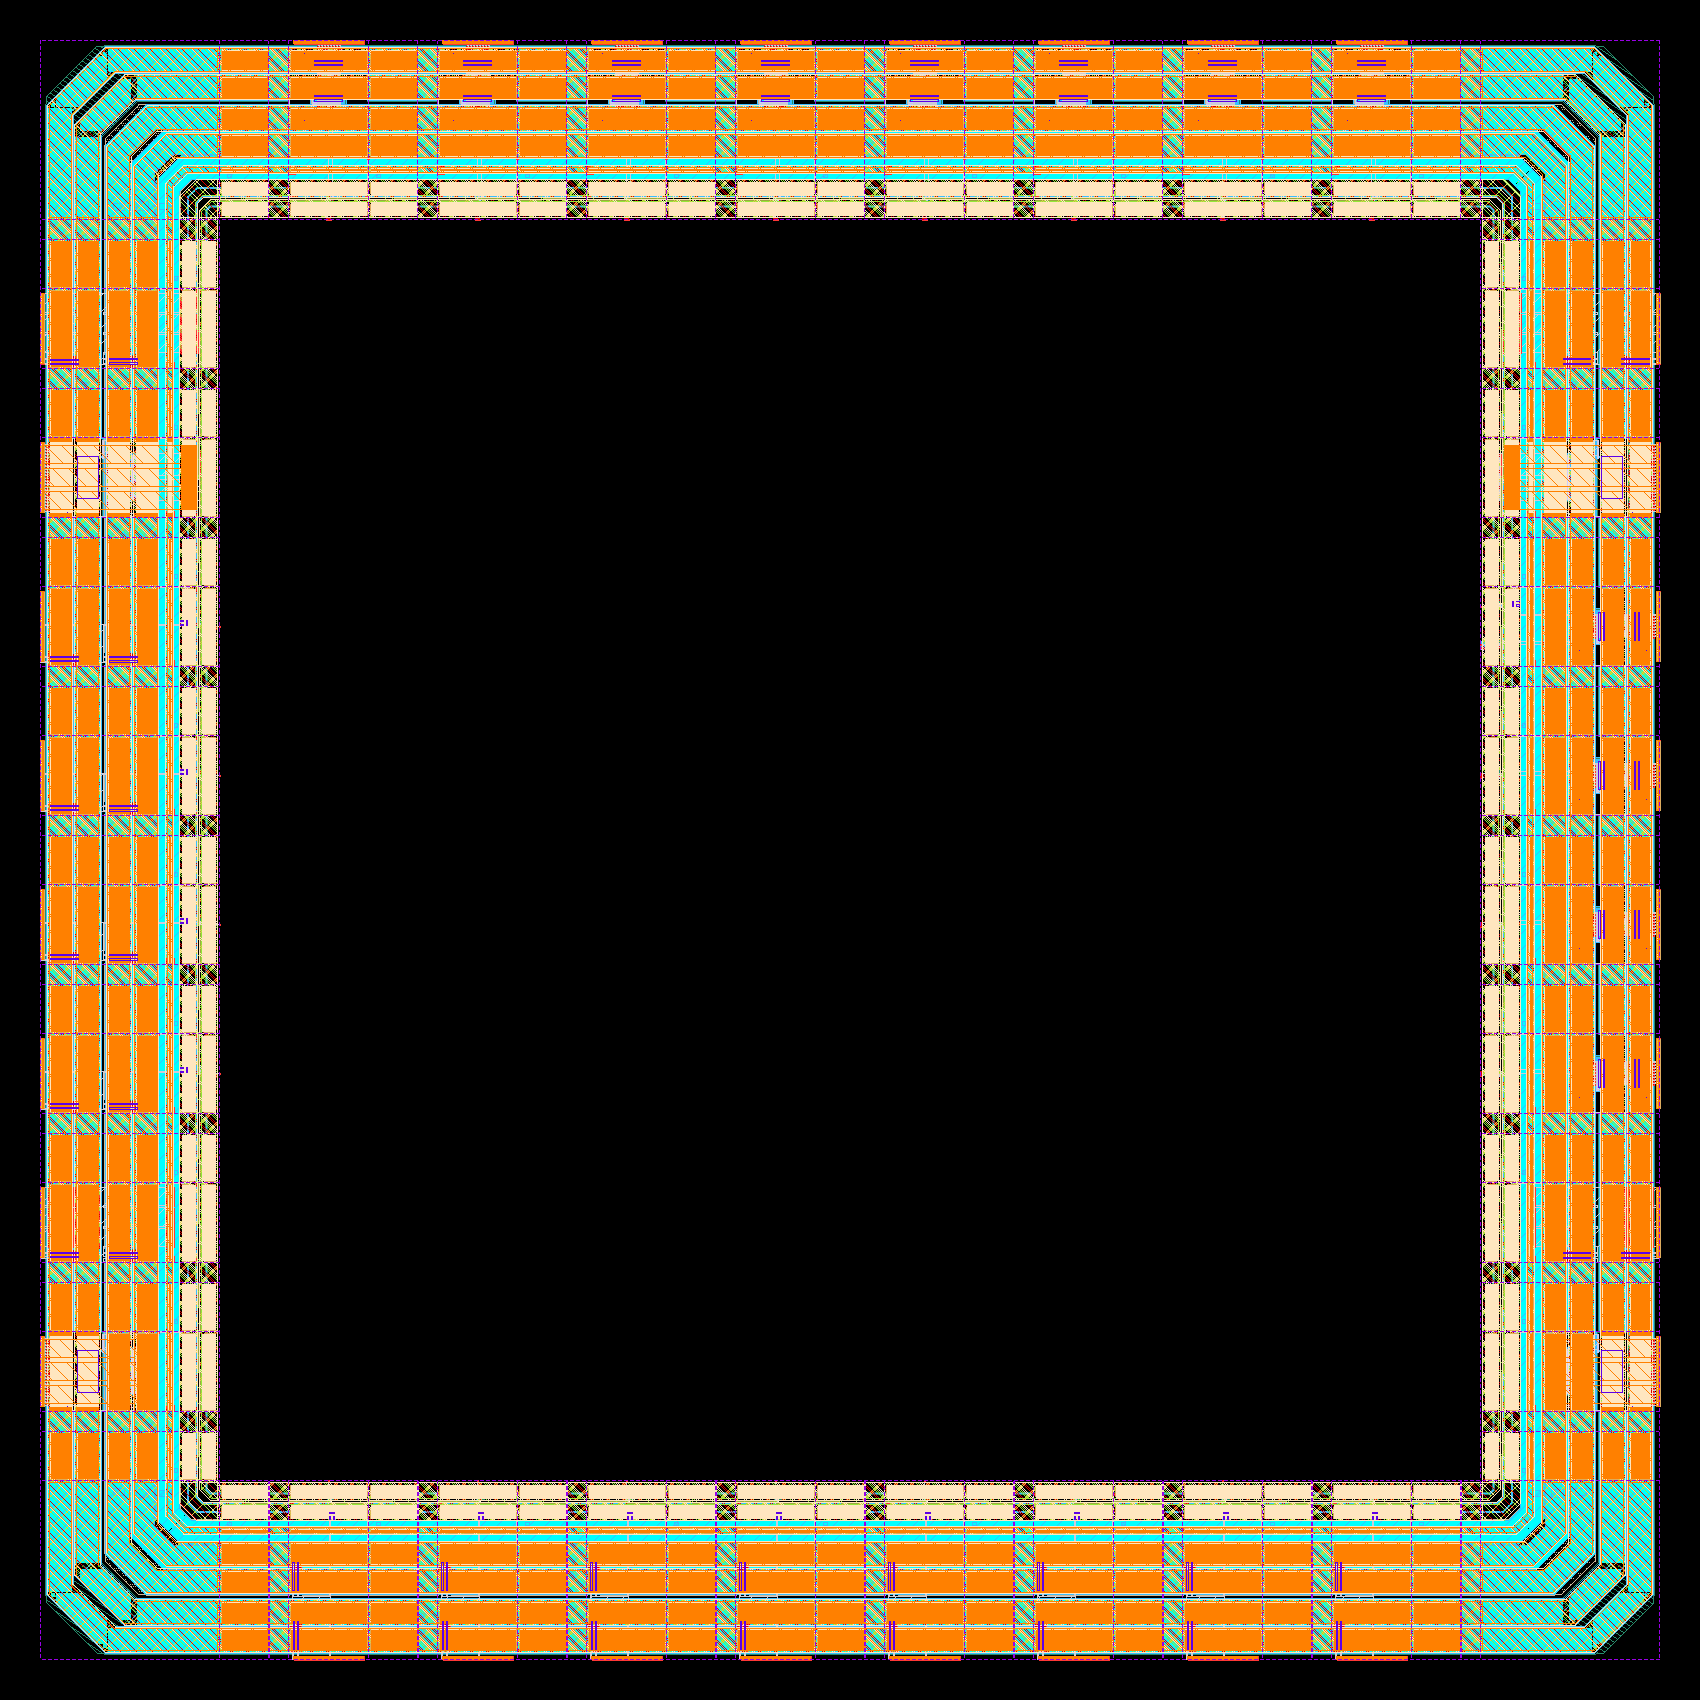
\includegraphics[width=0.82\textwidth,height=\textheight]{fig/padring_layout.png}
\caption{Generated \texttt{chip\_top} pad ring at \textbf{150 µm pad
pitch}, rendered from GDS with the IHP SG13G2 layer palette --- a fully
\emph{closed} ring: the four chamfered \texttt{sg13g2\_Corner} cells
turn the ring at the die corners, eight I/O pads occupy each side at 150
µm centre-to-centre spacing, and \texttt{sg13g2\_Filler*} cells tile the
70 µm gaps, so the supply and ESD rails run continuously around the die
(\texttt{connect\_by\_abutment}). Geometric check from the DEF: each
side is tiled gap-free from corner to corner (140 µm → 1770 µm). The
core area in the centre is empty because the flow was stopped at the
pad-ring step.}
\end{figure}

The same placement, coloured by pad \emph{function} rather than by mask
layer, makes the floor-planning choices explicit:

\begin{figure}
\centering
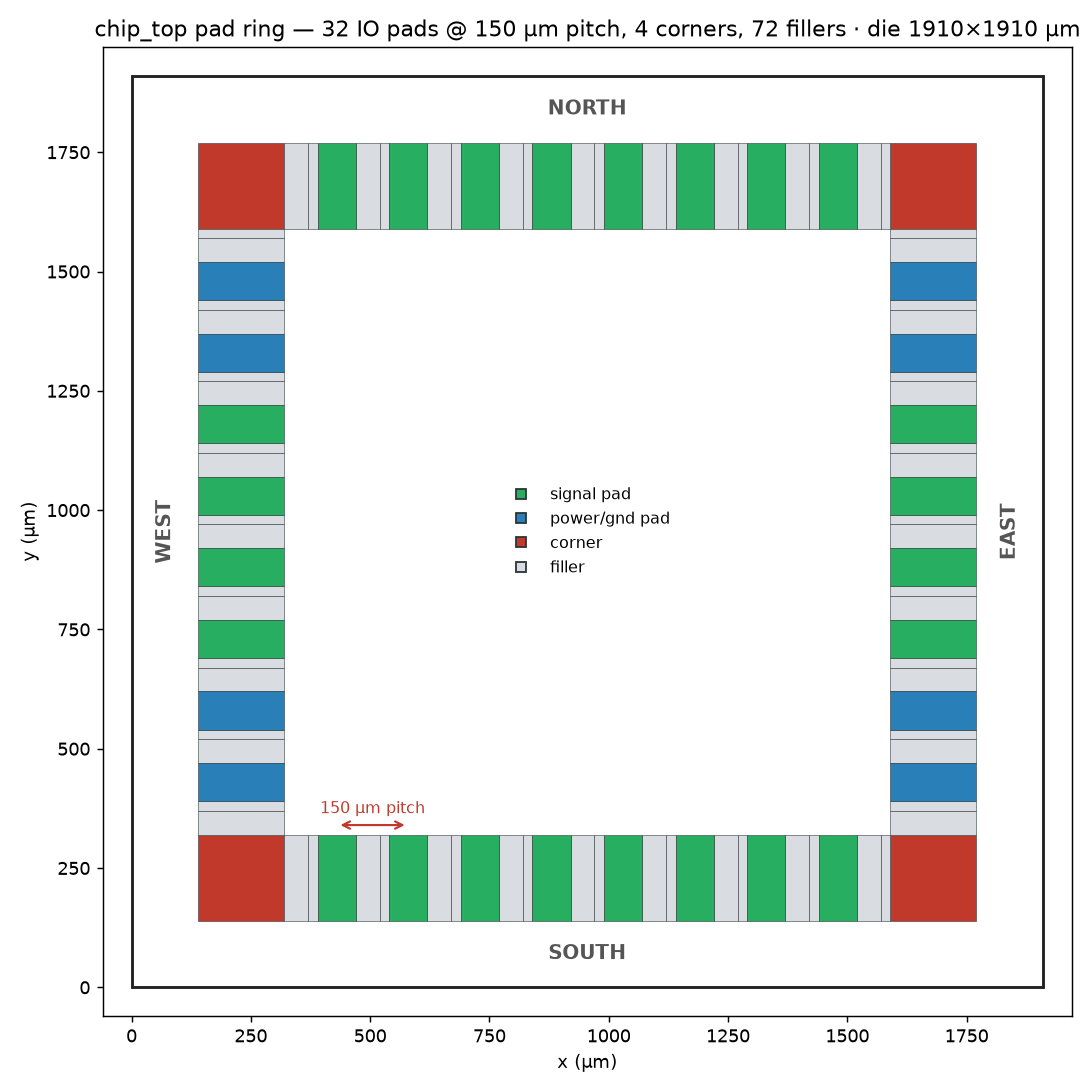
\includegraphics[width=0.7\textwidth,height=\textheight]{fig/padring_floorplan.png}
\caption{Pad-ring floor plan by function: green = signal pads, blue =
power/ground pads, red = corner cells, grey = fillers. 32 I/O pads at a
uniform 150 µm pitch + 4 corners + 72 fillers on a 1910 × 1910 µm die,
each pad inset 140 µm from the die edge to leave room for the seal
ring.}
\end{figure}

The placer's own report confirms the geometry: each side sums to
\textbf{640 µm} of pad width (8 × 80 µm), the free space is distributed
as an exact \textbf{70 µm} gap between pads
(\texttt{space\_between\_pads:\ 70.0}), and the run ends with
\emph{``Placing corner cells\ldots{} Placing filler cells\ldots{}
Connecting ring signals\ldots{}''} and \textbf{Flow complete}. A
centre-to-centre check on the emitted DEF gives a single pitch value of
\textbf{150.0 µm} on every side (pad centres at 430, 580, \ldots, 1480
µm). The DEF contains 32 I/O pads (12 inputs, 11 outputs, 1
bidirectional, 8 supply), 4 corners and 72 fillers on the 1910 × 1910 µm
die.

\begin{center}\rule{0.5\linewidth}{0.5pt}\end{center}

\hypertarget{verification-and-next-steps}{%
\section{8. Verification and next
steps}\label{verification-and-next-steps}}

\textbf{How to check the ring.} The fastest check is the
\texttt{pad\_cfg.tcl} console output: a \emph{``sum of cell widths
\ldots{} larger than the width of this side''} error means
\texttt{DIE\_AREA} is too small, and a \emph{``No instance \ldots{}
found''} error means a \texttt{PAD\_*} name does not match a Verilog
instance. Visually, open the run in the OpenROAD GUI ---
\texttt{librelane\ config.yaml\ -\/-pdk\ "\$PDK"\ -\/-pdk-root\ "\$PDK\_ROOT"\ -\/-manual-pdk\ -\/-last-run\ -f\ openinopenroad}
--- and confirm four populated sides, four corners, gap-free fillers,
and the 140 µm inset.

\textbf{From pad ring to chip.} Removing
\texttt{-\/-to\ OpenROAD.PadRing} runs the full \texttt{Chip} flow: it
places and routes the core inside the ring, generates the seal ring,
inserts fillers, and runs the density and antenna checks, ending in a
final chip GDS under \texttt{runs/…/final/gds/}.

\textbf{For your own core.} Replace the placeholder \texttt{demo\_core}
with the actual core RTL (or drop in a hardened core macro via
\texttt{MACROS}/\texttt{EXTRA\_LEFS}), then edit the pad instantiations
and the four \texttt{PAD\_*} lists to match its true pin-out and
drive-strength requirements --- the method itself does not change.

\begin{center}\rule{0.5\linewidth}{0.5pt}\end{center}

\hypertarget{appendix-a-reproduction}{%
\section{Appendix A --- reproduction}\label{appendix-a-reproduction}}

\begin{Shaded}
\begin{Highlighting}[]
\NormalTok{Design    : this repository (pad{-}ring{-}ihp)}
\NormalTok{Files     : src/chip\_top.v   chip top, instantiates the pad ring}
\NormalTok{            src/demo\_core.v        placeholder core}
\NormalTok{            config.yaml          flow = Chip, PAD\_* side lists, DIE\_AREA}
\NormalTok{            constraint.sdc       clock defined at the clock pad\textquotesingle{}s p2c pin}
\NormalTok{            env.sh               PDK\_ROOT / PDK, tool{-}path setup}
\NormalTok{            gen\_padring.sh      driver (see §4)}
\NormalTok{            scripts/render\_padring.py  DEF+GDS {-}\textgreater{} layout PNG (fig below)}
\NormalTok{Run       : ./gen\_padring.sh}
\NormalTok{PDK       : ihp{-}sg13g2 @ $PDK\_ROOT   (LibreLane 3.1, {-}{-}manual{-}pdk)}
\NormalTok{Output    : runs/RUN\_*/16{-}openroad{-}padring/chip\_top.def}
\NormalTok{Check     : scripts/check\_padring.py \textless{}def\textgreater{} {-}{-}pitch 150   (PASS required)}
\NormalTok{Figure    : doc/fig/padring\_layout.png  (GDS render, PDK colours)}
\NormalTok{            doc/fig/padring\_floorplan.png (function{-}coloured floor plan)}
\end{Highlighting}
\end{Shaded}

\begin{center}\rule{0.5\linewidth}{0.5pt}\end{center}

\hypertarget{appendix-b-third-party-tools-and-libraries}{%
\section{Appendix B --- Third-party tools and
libraries}\label{appendix-b-third-party-tools-and-libraries}}

All process-specific material in this project --- I/O cells, layer
stack, KLayout layer palette, LibreLane PDK configuration --- comes
exclusively from the \textbf{IHP SG13G2 open PDK}. No other foundry's
libraries, rules or documentation are used or referenced.

\textbf{Used to generate and verify the pad ring} (all invoked by
\texttt{gen\_padring.sh} / \texttt{scripts/}):

\begin{longtable}[]{@{}
  >{\raggedright\arraybackslash}p{(\columnwidth - 6\tabcolsep) * \real{0.2500}}
  >{\raggedright\arraybackslash}p{(\columnwidth - 6\tabcolsep) * \real{0.2500}}
  >{\raggedright\arraybackslash}p{(\columnwidth - 6\tabcolsep) * \real{0.2500}}
  >{\raggedright\arraybackslash}p{(\columnwidth - 6\tabcolsep) * \real{0.2500}}@{}}
\toprule\noalign{}
\begin{minipage}[b]{\linewidth}\raggedright
Tool / library
\end{minipage} & \begin{minipage}[b]{\linewidth}\raggedright
Version
\end{minipage} & \begin{minipage}[b]{\linewidth}\raggedright
License
\end{minipage} & \begin{minipage}[b]{\linewidth}\raggedright
Role
\end{minipage} \\
\midrule\noalign{}
\endhead
\bottomrule\noalign{}
\endlastfoot
\href{https://github.com/IHP-GmbH/IHP-Open-PDK}{IHP-Open-PDK}
(\texttt{ihp-sg13g2}) & commit \texttt{144f811c} & Apache-2.0 & Process
kit: \texttt{sg13g2\_io} pad cells (LEF/GDS/Verilog/Liberty),
\texttt{sg13g2\_stdcell}, LibreLane tech config, KLayout
\texttt{.lyp} \\
--- \texttt{sg13g2\_io} cell library & (in PDK) & Apache-2.0 & I/O pads,
corner and filler cells; generated from Chips4Makers
\href{https://gitlab.com/Chips4Makers/c4m-pdk-ihpsg13g2}{\texttt{c4m-pdk-ihpsg13g2}}
v0.0.4 plus contributed Liberty/Verilog views \\
\href{https://github.com/librelane/librelane}{LibreLane} & 3.1.0.dev1 &
Apache-2.0 & Flow engine: \texttt{Chip} flow, \texttt{OpenROAD.PadRing}
step, \texttt{pad\_cfg.tcl} placement algorithm \\
\href{https://github.com/The-OpenROAD-Project/OpenROAD}{OpenROAD} &
26Q2-2270-g4c26918f5 & BSD-3-Clause & Floorplan, ODB, built-in pad
placer (\texttt{make\_io\_sites}, \texttt{place\_pad},
\texttt{place\_corners}, \texttt{place\_io\_fill},
\texttt{connect\_by\_abutment}) \\
\href{https://github.com/YosysHQ/yosys}{Yosys} & 0.66 & ISC & Synthesis
of the chip top (pad instances kept via \texttt{(*\ keep\ *)}) \\
\href{https://www.klayout.de}{KLayout} (Python module) & 0.30.9 &
GPL-3.0-or-later & GDS assembly and headless rendering
(\texttt{scripts/render\_padring.py}) \\
\href{https://www.python.org}{Python} & 3.12.3 & PSF-2.0 & Scripts
(\texttt{check\_padring.py}, \texttt{render\_padring.py}, filters) \\
\end{longtable}

\textbf{Used to build this documentation} (\texttt{doc/build.sh}):

\begin{longtable}[]{@{}
  >{\raggedright\arraybackslash}p{(\columnwidth - 6\tabcolsep) * \real{0.2500}}
  >{\raggedright\arraybackslash}p{(\columnwidth - 6\tabcolsep) * \real{0.2500}}
  >{\raggedright\arraybackslash}p{(\columnwidth - 6\tabcolsep) * \real{0.2500}}
  >{\raggedright\arraybackslash}p{(\columnwidth - 6\tabcolsep) * \real{0.2500}}@{}}
\toprule\noalign{}
\begin{minipage}[b]{\linewidth}\raggedright
Tool / library
\end{minipage} & \begin{minipage}[b]{\linewidth}\raggedright
Version
\end{minipage} & \begin{minipage}[b]{\linewidth}\raggedright
License
\end{minipage} & \begin{minipage}[b]{\linewidth}\raggedright
Role
\end{minipage} \\
\midrule\noalign{}
\endhead
\bottomrule\noalign{}
\endlastfoot
\href{https://pandoc.org}{Pandoc} & 3.1.3 & GPL-2.0-or-later & Markdown
→ LaTeX conversion (default LaTeX template) \\
\href{https://tectonic-typesetting.github.io}{Tectonic} & 0.15.0 & MIT &
XeTeX-based LaTeX engine, LaTeX → PDF (any of
tectonic/xelatex/lualatex/pdflatex works) \\
\href{https://matplotlib.org}{Matplotlib} & 3.11.0 & Matplotlib License
(BSD-style) & Floor-plan figure generation \\
\end{longtable}

Notes:

\begin{itemize}
\tightlist
\item
  The full \texttt{Chip} flow (beyond the \texttt{OpenROAD.PadRing}
  stop) additionally uses \textbf{Magic}, \textbf{Netgen} and the
  \textbf{KLayout DRC/LVS decks} from the IHP PDK --- all open-source,
  none foundry-encumbered beyond the IHP PDK itself.
\item
  The \texttt{Verilator.Lint} step is disabled in \texttt{config.yaml}
  and Verilator is therefore not used.
\item
  The report is plain Markdown compiled to PDF via pandoc's default
  LaTeX template --- no custom template, stylesheet or filter is used.
\end{itemize}

\end{document}
